%==============================================================================
%  Exercise 2 --- Thống kê nhiều chiều & cao chiều (Chương 3)
%  Theo templates/hmmt-solution-template.tex (phong cách Harvard-MIT Math Tournament)
%  - Chỉ trắng và đen: không màu, không khung, không tcolorbox, không đổ bóng.
%  - Tiêu đề gọn ở giữa trang, không trang bìa, không \maketitle.
%  - Đề bài chạy dòng ("1." / "Bài 2.1." in đậm), lời giải run-in "Lời giải:".
%  - Đáp số cuối cùng đóng khung bằng \boxed{...}.
%  Biên dịch: xelatex (bắt buộc, vì dùng fontspec + polyglossia + unicode-math)
%==============================================================================
\documentclass[11pt,a4paper]{article}

% --- Ngôn ngữ và font: Latin Modern (Computer Modern) như bản HMMT gốc -------
\usepackage{fontspec}
\usepackage{polyglossia}
\setdefaultlanguage{vietnamese}
\setmainfont{lmroman10-regular.otf}[
  BoldFont       = lmroman10-bold.otf,
  ItalicFont     = lmroman10-italic.otf,
  BoldItalicFont = lmroman10-bolditalic.otf
]

% --- Toán học ---------------------------------------------------------------
\usepackage{amsmath, amssymb, amsthm}
\usepackage{unicode-math}
\setmathfont{latinmodern-math.otf}
\renewcommand{\boldsymbol}[1]{\symbf{#1}}
% Giữ nguyên từng khối tính toán, không ngắt giữa các dòng align.

% --- Khổ trang: lề rộng, khối chữ gọn vào giữa ------------------------------
\usepackage[a4paper, top=2.5cm, bottom=2.5cm, left=2.7cm, right=2.7cm]{geometry}
\usepackage{enumitem}
\usepackage{graphicx}
\usepackage{booktabs}
\setlist{itemsep=5pt, topsep=6pt, parsep=2pt, partopsep=0pt, leftmargin=1.8em}

% Đoạn văn kiểu HMMT: thụt đầu dòng, KHÔNG dùng parskip (không chèn dòng trống)
\setlength{\parindent}{1.5em}
\setlength{\parskip}{0pt}
\setlength{\abovedisplayskip}{5pt plus 1pt minus 2pt}
\setlength{\belowdisplayskip}{5pt plus 1pt minus 2pt}
\setlength{\abovedisplayshortskip}{2pt plus 1pt}
\setlength{\belowdisplayshortskip}{2pt plus 1pt}

% Chỉ số trang canh giữa chân trang, không running header
\pagestyle{plain}
\raggedbottom
\clubpenalty=10000
\widowpenalty=10000

% --- Thông tin tài liệu (sửa 4 dòng này cho mỗi bài) ------------------------
\newcommand{\coursename}{Thống kê nhiều chiều}
\newcommand{\docdate}{\today}
\newcommand{\doctitle}{Lời giải bài tập về nhà -- Exercise 2}
\newcommand{\studentname}{Quang Nguyễn}

% --- Đề bài / lời giải ------------------------------------------------------
\newcounter{prob}
\makeatletter
% \begin{problem}            -> tự đánh số 1., 2., 3., ...
% \begin{problem}[Bài 2.1.]  -> dùng nhãn tự đặt
\newenvironment{problem}[1][]{%
  \par\addvspace{14pt}\noindent\begin{minipage}{\linewidth}
  \def\@tempa{#1}%
  \ifx\@tempa\@empty\refstepcounter{prob}\textbf{\theprob.}\else\textbf{#1}\fi
  \ \ignorespaces
}{\par\end{minipage}\par\nopagebreak[4]}
\makeatother

% Lời giải: tiêu đề riêng dòng, tách rõ khỏi các ý của đề bài.
\newenvironment{solution}{%
  \par\medskip\noindent\textbf{Lời giải:}\par\nobreak\smallskip\noindent\ignorespaces
}{\par}

% Đáp số cuối cùng luôn đóng khung
\newcommand{\answer}[1]{\boxed{#1}}
% Mỗi câu có các bước riêng; giữ tiêu đề bước cùng phần giải thích tiếp theo.
\newcommand{\step}[2]{\par\medskip\noindent\textbf{Bước #1. #2}\par\nopagebreak[4]\smallskip\noindent}


\begin{document}

%------------------------------ Tiêu đề gọn ---------------------------------
\begin{center}
  {\bfseries\coursename}\\
  \docdate\\
  \doctitle: \textbf{\studentname}
\end{center}
\vspace{0.5em}

\begin{problem}[Bài 3.1.]
Cho ma trận dữ liệu
\[
\mathbf{X}=\begin{pmatrix}2&12\\8&9\\6&9\\8&10\end{pmatrix}.
\]
\begin{enumerate}[label=(\alph*)]
\item Tính $T^2$ để kiểm định $H_0:\boldsymbol{\mu}=(7,11)'$.

\item Xác định phân phối của $T^2$ ở câu (a).

\item Kiểm định $H_0$ ở mức ý nghĩa $\alpha=0.05$.
\end{enumerate}
\end{problem}
\begin{solution}
Quy ước: $G(\gamma)$ là phân vị mức $\gamma$ của phân phối $G$,
tức $P(Z\le G(\gamma))=\gamma$ khi $Z\sim G$.
Các kết quả Hotelling chính xác dưới giả thiết các quan sát độc lập,
cùng phân phối chuẩn hai chiều và hiệp phương sai xác định dương.
\begin{enumerate}[label=\textbf{\alph*)}]
\item \textbf{Tính thống kê Hotelling.}\par\nopagebreak[4]
\step{1}{Xác định công thức và các đại lượng phải tính.}
Có $n=4$ hàng quan sát, $p=2$ biến và $\boldsymbol{\mu}_0=(7,11)'$.
Công thức là
\[
T^2=n\mathbf{d}'\mathbf{S}^{-1}\mathbf{d},\qquad
\mathbf{d}=\bar{\mathbf{x}}-\boldsymbol{\mu}_0.
\]
Cần tính lần lượt $\bar{\mathbf{x}}$, $\mathbf{S}$, $\mathbf{S}^{-1}$ và $\mathbf{d}$.
Ở đây $\mathbf{S}$ là hiệp phương sai mẫu với mẫu số $n-1$.
\step{2}{Tính trung bình và sai lệch từng quan sát.}
\begin{align*}
\bar{x}_1&=\frac{2+8+6+8}{4}=\frac{24}{4}=6,\\
\bar{x}_2&=\frac{12+9+9+10}{4}=\frac{40}{4}=10.
\end{align*}
Trừ trung bình từng cột:
\[
\mathbf{X}_c=\begin{pmatrix}
2-6&12-10\\8-6&9-10\\6-6&9-10\\8-6&10-10
\end{pmatrix}
=\begin{pmatrix}-4&2\\2&-1\\0&-1\\2&0\end{pmatrix}.
\]
\step{3}{Tính từng phần tử của hiệp phương sai mẫu.}
Công thức chung:
\[
s_{jk}=\frac1{n-1}\sum_{i=1}^n(x_{ij}-\bar{x}_j)(x_{ik}-\bar{x}_k).
\]
Thế các sai lệch ở Bước 2:
\begin{align*}
s_{11}&=\frac{(-4)^2+2^2+0^2+2^2}{3}
=\frac{16+4+0+4}{3}=8,\\
s_{22}&=\frac{2^2+(-1)^2+(-1)^2+0^2}{3}
=\frac{4+1+1+0}{3}=2,\\
s_{12}&=\frac{(-4)2+2(-1)+0(-1)+2\cdot0}{3}
=\frac{-8-2+0+0}{3}=-\frac{10}{3}.
\end{align*}
Vì $s_{21}=s_{12}$,
\[
\mathbf{S}=\begin{pmatrix}8&-10/3\\-10/3&2\end{pmatrix}.
\]
\step{4}{Tính định thức và nghịch đảo.}
Dùng công thức
\[
\begin{pmatrix}a&b\\b&c\end{pmatrix}^{-1}
=\frac1{ac-b^2}\begin{pmatrix}c&-b\\-b&a\end{pmatrix}.
\]
Ở đây $a=8$, $b=-10/3$, $c=2$, nên
\begin{align*}
\det\mathbf{S}&=8\cdot2-(-10/3)^2
=16-\frac{100}{9}=\frac{44}{9}>0,\\
\mathbf{S}^{-1}&=\frac9{44}\begin{pmatrix}2&10/3\\10/3&8\end{pmatrix}.
\end{align*}
Các phần tử lần lượt là $18/44=9/22$, $30/44=15/22$,
$30/44=15/22$, $72/44=36/22$, do đó
\[
\mathbf{S}^{-1}=\frac1{22}\begin{pmatrix}9&15\\15&36\end{pmatrix}.
\]
\step{5}{Tính dạng toàn phương qua hai phép nhân.}
Trước hết
\[
\mathbf{d}=\begin{pmatrix}6-7\\10-11\end{pmatrix}
=\begin{pmatrix}-1\\-1\end{pmatrix}.
\]
Tiếp theo
\begin{align*}
\mathbf{S}^{-1}\mathbf{d}
&=\frac1{22}\begin{pmatrix}9(-1)+15(-1)\\15(-1)+36(-1)\end{pmatrix}
=\frac1{22}\begin{pmatrix}-24\\-51\end{pmatrix},\\
\mathbf{d}'(\mathbf{S}^{-1}\mathbf{d})
&=\frac{(-1)(-24)+(-1)(-51)}{22}
=\frac{24+51}{22}=\frac{75}{22},\\
T^2&=4\cdot\frac{75}{22}=\frac{300}{22}.
\end{align*}
\textbf{Kết quả:} $\displaystyle\answer{T^2=\frac{150}{11}\approx13.6364}$.
\item \textbf{Phân phối dưới $H_0$.}\par\nopagebreak[4]
\step{1}{Chọn định lý và kiểm tra kích thước.}
Dưới giả thiết mẫu chuẩn và $H_0$, với $n>p$,
\[
\frac{n-p}{p(n-1)}T^2\sim F_{p,n-p}.
\]
Ở đây $4>2$, nên áp dụng được.
\step{2}{Tính hệ số và bậc tự do.}
\begin{align*}
n-p&=4-2=2,\\
p(n-1)&=2(4-1)=6,\\
\frac{n-p}{p(n-1)}&=\frac26=\frac13.
\end{align*}
\step{3}{Kết luận.}
\[
\answer{\frac{T^2}{3}\sim F_{2,2}\quad\text{khi }H_0\text{ đúng}.}
\]
\item \textbf{Kiểm định ở mức $5\%$.}\par\nopagebreak[4]
\step{1}{Xác định giả thuyết và ngưỡng phân vị.}
$H_0:\boldsymbol{\mu}=(7,11)'$, $H_1:\boldsymbol{\mu}\ne(7,11)'$.
Thống kê $T^2$ đo độ lệch nên bác bỏ khi giá trị lớn.
Mức $\alpha=0.05$ cho phân vị $1-\alpha=0.95$.
\step{2}{Tính ngưỡng bác bỏ.}
Công thức là $c=\frac{p(n-1)}{n-p}F_{p,n-p}(1-\alpha)$.
Đối với $F_{2,2}$, hàm phân phối là $P(F\le x)=x/(1+x)$, $x\ge0$.
Để tìm phân vị $q$:
\begin{align*}
\frac{q}{1+q}&=0.95,\\
q&=0.95+0.95q,\\
0.05q&=0.95,\qquad q=19.
\end{align*}
Do đó
\[
c=\frac{2(4-1)}{4-2}\cdot19=\frac62\cdot19=57.
\]
\step{3}{So sánh và kiểm tra bằng p-value.}
$T^2_{\mathrm{obs}}=150/11\approx13.6364<57$.
Thống kê đã đổi về phân phối $F$ là
\[
F_{\mathrm{obs}}=\frac13\frac{150}{11}=\frac{50}{11}.
\]
Dùng hàm phân phối ở Bước 2:
\begin{align*}
\text{p-value}&=P(F_{2,2}\ge F_{\mathrm{obs}})
=1-\frac{F_{\mathrm{obs}}}{1+F_{\mathrm{obs}}}\\
&=\frac1{1+50/11}=\frac{11}{61}\approx0.1803>0.05.
\end{align*}
\step{4}{Kết luận.}
\textbf{Chưa bác bỏ $H_0$ ở mức $5\%$}. Chưa có đủ bằng chứng rằng
vectơ trung bình khác $(7,11)'$.
\end{enumerate}
\end{solution}

\begin{problem}[Bài 3.2.]
Cho
\[
\mathbf{X}=\begin{pmatrix}6&9\\10&6\\8&3\end{pmatrix},\qquad
\mathbf{C}=\begin{pmatrix}1&-1\\1&1\end{pmatrix}.
\]
\begin{enumerate}[label=(\alph*)]
\item Tính $T^2$.
\item Biến đổi từng quan sát $\mathbf{x}_j$ thành $\mathbf{C}\mathbf{x}_j$
và xác định ma trận dữ liệu $\mathbf{Y}$.
\item Tính $T^2$ từ $\mathbf{Y}$ và so sánh với câu (a).
\end{enumerate}
\end{problem}
\begin{solution}
\textit{Đề không nêu vectơ trung bình giả thuyết $\boldsymbol{\mu}_0$.
Ta giải tổng quát với $\boldsymbol{\mu}_0=(a,b)'$, là giá trị giả thuyết
được chỉ định trước. Dữ liệu không xác định $\boldsymbol{\mu}_0$;
vì vậy chưa có một đáp số số học duy nhất.}
\begin{enumerate}[label=\textbf{\alph*)}]
\item \textbf{Tính $T_X^2$ từ dữ liệu ban đầu.}\par\nopagebreak[4]
\step{1}{Xác định công thức.}
Có $n=3$, $p=2$. Cần tính $\bar{\mathbf{x}}$, $\mathbf{S}_X$ và nghịch đảo,
sau đó dùng $T_X^2=3\mathbf{d}_X'\mathbf{S}_X^{-1}\mathbf{d}_X$,
với $\mathbf{d}_X=\bar{\mathbf{x}}-\boldsymbol{\mu}_0$.
\step{2}{Tính trung bình và dữ liệu trừ trung bình.}
\begin{align*}
\bar{x}_1&=\frac{6+10+8}{3}=\frac{24}{3}=8,\\
\bar{x}_2&=\frac{9+6+3}{3}=\frac{18}{3}=6.
\end{align*}
Do đó
\[
\mathbf{X}_c=\begin{pmatrix}6-8&9-6\\10-8&6-6\\8-8&3-6\end{pmatrix}
=\begin{pmatrix}-2&3\\2&0\\0&-3\end{pmatrix}.
\]
\step{3}{Tính từng hiệp phương sai.}
Dùng $s_{jk}=(n-1)^{-1}\sum_i(x_{ij}-\bar{x}_j)(x_{ik}-\bar{x}_k)$:
\begin{align*}
s_{11}&=\frac{(-2)^2+2^2+0^2}{2}=\frac{4+4}{2}=4,\\
s_{22}&=\frac{3^2+0^2+(-3)^2}{2}=\frac{9+9}{2}=9,\\
s_{12}&=\frac{(-2)3+2\cdot0+0(-3)}{2}=\frac{-6}{2}=-3.
\end{align*}
Vậy $\mathbf{S}_X=\begin{pmatrix}4&-3\\-3&9\end{pmatrix}$.
\step{4}{Tính nghịch đảo.}
Dùng công thức nghịch đảo $2\times2$ ở Bài 3.1:
\begin{align*}
\det\mathbf{S}_X&=4\cdot9-(-3)^2=36-9=27,\\
\mathbf{S}_X^{-1}&=\frac1{27}\begin{pmatrix}9&3\\3&4\end{pmatrix}.
\end{align*}
Các phần tử nghịch đảo là $9/27$, $3/27$, $3/27$, $4/27$.
\step{5}{Tính dạng toàn phương tổng quát.}
Đặt $u=8-a$, $v=6-b$, do đó $\mathbf{d}_X=(u,v)'$.
\begin{align*}
\mathbf{S}_X^{-1}\mathbf{d}_X
&=\frac1{27}\begin{pmatrix}9u+3v\\3u+4v\end{pmatrix},\\
\mathbf{d}_X'\mathbf{S}_X^{-1}\mathbf{d}_X
&=\frac1{27}\{u(9u+3v)+v(3u+4v)\}\\
&=\frac1{27}(9u^2+3uv+3uv+4v^2),\\
T_X^2&=\frac3{27}(9u^2+6uv+4v^2).
\end{align*}
\[
\answer{T_X^2=\frac19(9u^2+6uv+4v^2)}.
\]
\step{6}{Minh họa với hai giả định riêng biệt.}
\emph{Giả định 1:} nếu chọn $\boldsymbol{\mu}_0=(7,11)'$ như Bài 3.1,
$u=8-7=1$, $v=6-11=-5$. Tính từng hạng tử:
\begin{align*}
9u^2&=9(1)^2=9,\\
6uv&=6(1)(-5)=-30,\\
4v^2&=4(-5)^2=100,\\
T_X^2&=\frac{9-30+100}{9}=\answer{\frac{79}{9}\approx8.7778}.
\end{align*}
\emph{Giả định 2:} nếu chọn $\boldsymbol{\mu}_0=\mathbf{0}$,
$u=8$, $v=6$. Khi đó
\begin{align*}
9u^2&=9\cdot64=576,\\
6uv&=6\cdot8\cdot6=288,\\
4v^2&=4\cdot36=144,\\
T_X^2&=\frac{576+288+144}{9}=\frac{1008}{9}=\answer{112}.
\end{align*}
\item \textbf{Biến đổi dữ liệu.}\par\nopagebreak[4]
\step{1}{Tính từng quan sát theo công thức.}
Với $\mathbf{x}_i=(x_{i1},x_{i2})'$,
\[
\mathbf{y}_i=\mathbf{C}\mathbf{x}_i
=\begin{pmatrix}x_{i1}-x_{i2}\\x_{i1}+x_{i2}\end{pmatrix}.
\]
Thế lần lượt ba quan sát:
\begin{align*}
\mathbf{y}_1&=\begin{pmatrix}6-9\\6+9\end{pmatrix}
=\begin{pmatrix}-3\\15\end{pmatrix},\\
\mathbf{y}_2&=\begin{pmatrix}10-6\\10+6\end{pmatrix}
=\begin{pmatrix}4\\16\end{pmatrix},\\
\mathbf{y}_3&=\begin{pmatrix}8-3\\8+3\end{pmatrix}
=\begin{pmatrix}5\\11\end{pmatrix}.
\end{align*}
Trong công thức $\mathbf{y}_i=\mathbf{C}\mathbf{x}_i$, mỗi quan sát là
\emph{vectơ cột}. Còn hàng thứ $i$ của ma trận dữ liệu là $\mathbf{x}_i'$.
Chuyển vị cả hai vế, dùng quy tắc $(\mathbf{A}\mathbf{B})'
=\mathbf{B}'\mathbf{A}'$, ta có
\[
\mathbf{y}_i'=(\mathbf{C}\mathbf{x}_i)'=\mathbf{x}_i'\mathbf{C}'.
\]
Ghép các hàng $\mathbf{y}_i'$ thành ma trận dữ liệu mới, suy ra
\[
\answer{\mathbf{Y}=\mathbf{X}\mathbf{C}'
=\begin{pmatrix}-3&15\\4&16\\5&11\end{pmatrix}}.
\]
\step{2}{Tính trung bình và sai lệch của dữ liệu mới.}
\begin{align*}
\bar{y}_1&=\frac{-3+4+5}{3}=2,\\
\bar{y}_2&=\frac{15+16+11}{3}=14.
\end{align*}
Suy ra $\bar{\mathbf{y}}=(2,14)'$ và
\[
\mathbf{Y}_c=\begin{pmatrix}-3-2&15-14\\4-2&16-14\\5-2&11-14\end{pmatrix}
=\begin{pmatrix}-5&1\\2&2\\3&-3\end{pmatrix}.
\]
\step{3}{Tính hiệp phương sai và nghịch đảo từ dữ liệu mới.}
\begin{align*}
s_{Y,11}&=\frac{(-5)^2+2^2+3^2}{2}=\frac{25+4+9}{2}=19,\\
s_{Y,22}&=\frac{1^2+2^2+(-3)^2}{2}=\frac{1+4+9}{2}=7,\\
s_{Y,12}&=\frac{(-5)1+2\cdot2+3(-3)}{2}=\frac{-5+4-9}{2}=-5,\\
\det\mathbf{S}_Y&=19\cdot7-(-5)^2=133-25=108.
\end{align*}
Do đó
\[
\mathbf{S}_Y=\begin{pmatrix}19&-5\\-5&7\end{pmatrix},\qquad
\mathbf{S}_Y^{-1}=\frac1{108}\begin{pmatrix}7&5\\5&19\end{pmatrix}.
\]
\step{4}{Làm rõ quy tắc nhân ma trận trước khi kiểm tra.}
Với tích $\mathbf{A}\mathbf{B}$, luôn lấy \textbf{hàng của ma trận bên trái}
nhân với \textbf{cột của ma trận bên phải}. Phần tử hàng $i$, cột $j$ là
\[
(\mathbf{A}\mathbf{B})_{ij}=\sum_{k=1}^q A_{ik}B_{kj}.
\]
Điều kiện kích thước: nếu $\mathbf{A}$ có kích thước $m\times q$ và
$\mathbf{B}$ có kích thước $q\times r$, thì tích có kích thước $m\times r$.
Số cột của ma trận bên trái phải bằng số hàng của ma trận bên phải.

Ví dụ với chính phép biến đổi của bài, lấy hàng 1 của $\mathbf{C}$
nhân cột $\mathbf{x}_1=(6,9)'$:
\[
(\mathbf{C}\mathbf{x}_1)_1=(1,-1)\begin{pmatrix}6\\9\end{pmatrix}
=1\cdot6+(-1)\cdot9=-3.
\]
Hàng 2 cho $(\mathbf{C}\mathbf{x}_1)_2=1\cdot6+1\cdot9=15$.

Với ba ma trận, \textbf{được chọn cặp nào tính trước, nhưng phải giữ nguyên
thứ tự các ma trận}. Đây là tính kết hợp:
\[
\boxed{(\mathbf{A}\mathbf{B})\mathbf{D}
=\mathbf{A}(\mathbf{B}\mathbf{D}).}
\]
Tính kết hợp không cho phép đổi chỗ hai ma trận:
nói chung $\mathbf{A}\mathbf{B}\ne\mathbf{B}\mathbf{A}$.
Vì vậy không có quy định chung rằng phải tính tích ma trận từ trái sang phải
hay từ phải sang trái; cần phân biệt \emph{cách đặt ngoặc} với
\emph{thứ tự các thừa số}.

\step{5}{Suy ra vì sao công thức là $\mathbf{C}\mathbf{S}_X\mathbf{C}'$.}
Đề cho $\mathbf{y}_i=\mathbf{C}\mathbf{x}_i$, nên
$\bar{\mathbf{y}}=\mathbf{C}\bar{\mathbf{x}}$.
Đặt các vectơ sai lệch
\[
\mathbf{d}_i=\mathbf{x}_i-\bar{\mathbf{x}},\qquad
\mathbf{e}_i=\mathbf{y}_i-\bar{\mathbf{y}}.
\]
Khi đó
\[
\mathbf{e}_i=\mathbf{C}\mathbf{x}_i-\mathbf{C}\bar{\mathbf{x}}
=\mathbf{C}(\mathbf{x}_i-\bar{\mathbf{x}})=\mathbf{C}\mathbf{d}_i.
\]
Theo định nghĩa hiệp phương sai mẫu,
\[
\mathbf{S}_X=\frac1{n-1}\sum_{i=1}^n\mathbf{d}_i\mathbf{d}_i',\qquad
\mathbf{S}_Y=\frac1{n-1}\sum_{i=1}^n\mathbf{e}_i\mathbf{e}_i'.
\]
Thế $\mathbf{e}_i=\mathbf{C}\mathbf{d}_i$ vào công thức thứ hai.
Điểm cần chú ý là \textbf{chuyển vị của tích phải đảo thứ tự}:
\[
(\mathbf{C}\mathbf{d}_i)'=\mathbf{d}_i'\mathbf{C}'.
\]
Do đó
\begin{align*}
\mathbf{S}_Y
&=\frac1{n-1}\sum_{i=1}^n
 (\mathbf{C}\mathbf{d}_i)(\mathbf{C}\mathbf{d}_i)'\\
&=\frac1{n-1}\sum_{i=1}^n
 \mathbf{C}\mathbf{d}_i\mathbf{d}_i'\mathbf{C}'\\
&=\mathbf{C}\left(\frac1{n-1}\sum_{i=1}^n
 \mathbf{d}_i\mathbf{d}_i'\right)\mathbf{C}'\\
&=\boxed{\mathbf{C}\mathbf{S}_X\mathbf{C}'}.
\end{align*}
Ở bước đưa ra ngoài tổng, $\mathbf{C}$ vẫn ở bên trái và $\mathbf{C}'$
vẫn ở bên phải; ta không đổi vị trí hai ma trận.

Cũng có thể kiểm tra từ ma trận dữ liệu viết theo hàng.
Vì $\mathbf{Y}_c=\mathbf{X}_c\mathbf{C}'$ nên
\begin{align*}
\mathbf{S}_Y
&=\frac1{n-1}\mathbf{Y}_c'\mathbf{Y}_c\\
&=\frac1{n-1}(\mathbf{X}_c\mathbf{C}')'
                  (\mathbf{X}_c\mathbf{C}')\\
&=\frac1{n-1}\mathbf{C}\mathbf{X}_c'\mathbf{X}_c\mathbf{C}'
=\mathbf{C}\mathbf{S}_X\mathbf{C}'.
\end{align*}
Như vậy $\mathbf{Y}=\mathbf{X}\mathbf{C}'$ và
$\mathbf{S}_Y=\mathbf{C}\mathbf{S}_X\mathbf{C}'$ hoàn toàn nhất quán.

\step{6}{Kiểm tra số bằng cả hai cách đặt ngoặc.}
Các ma trận cần dùng là
\[
\mathbf{C}=\begin{pmatrix}1&-1\\1&1\end{pmatrix},\qquad
\mathbf{S}_X=\begin{pmatrix}4&-3\\-3&9\end{pmatrix},\qquad
\mathbf{C}'=\begin{pmatrix}1&1\\-1&1\end{pmatrix}.
\]
\textit{Cách 1: tính cặp bên trái trước, $(\mathbf{C}\mathbf{S}_X)\mathbf{C}'$.}
Theo quy tắc hàng nhân cột:
\begin{align*}
\mathbf{C}\mathbf{S}_X
&=\begin{pmatrix}
1\cdot4+(-1)(-3)&1(-3)+(-1)9\\
1\cdot4+1(-3)&1(-3)+1\cdot9
\end{pmatrix}\\
&=\begin{pmatrix}7&-12\\1&6\end{pmatrix}.
\end{align*}
Tiếp tục nhân kết quả bên trái với $\mathbf{C}'$ bên phải:
\begin{align*}
(\mathbf{C}\mathbf{S}_X)\mathbf{C}'
&=\begin{pmatrix}
7\cdot1+(-12)(-1)&7\cdot1+(-12)\cdot1\\
1\cdot1+6(-1)&1\cdot1+6\cdot1
\end{pmatrix}\\
&=\begin{pmatrix}19&-5\\-5&7\end{pmatrix}.
\end{align*}
\textit{Cách 2: tính cặp bên phải trước, $\mathbf{C}(\mathbf{S}_X\mathbf{C}')$.}
Vẫn lấy hàng của ma trận bên trái trong cặp nhân cột của ma trận bên phải:
\begin{align*}
\mathbf{S}_X\mathbf{C}'
&=\begin{pmatrix}
4\cdot1+(-3)(-1)&4\cdot1+(-3)\cdot1\\
(-3)\cdot1+9(-1)&(-3)\cdot1+9\cdot1
\end{pmatrix}\\
&=\begin{pmatrix}7&1\\-12&6\end{pmatrix}.
\end{align*}
Sau đó đặt $\mathbf{C}$ bên trái kết quả vừa tính:
\begin{align*}
\mathbf{C}(\mathbf{S}_X\mathbf{C}')
&=\begin{pmatrix}
1\cdot7+(-1)(-12)&1\cdot1+(-1)6\\
1\cdot7+1(-12)&1\cdot1+1\cdot6
\end{pmatrix}\\
&=\begin{pmatrix}19&-5\\-5&7\end{pmatrix}.
\end{align*}
Hai cách có kết quả trung gian khác nhau nhưng cùng kết quả cuối:
\[
\answer{\mathbf{S}_Y=\begin{pmatrix}19&-5\\-5&7\end{pmatrix}}.
\]
Kết quả này trùng với cách tính trực tiếp từ dữ liệu ở Bước 3.

\step{7}{Phân biệt với $\mathbf{C}'\mathbf{S}_X\mathbf{C}$ và thứ tự tác động.}
Nếu định nghĩa một biến đổi khác là $\mathbf{z}_i=\mathbf{C}'\mathbf{x}_i$,
thì công thức hiệp phương sai sẽ là
\[
\mathbf{S}_Z=\mathbf{C}'\mathbf{S}_X(\mathbf{C}')'
=\mathbf{C}'\mathbf{S}_X\mathbf{C}.
\]
Hai biến đổi khác nhau ngay ở thành phần của vectơ:
\[
\mathbf{C}\mathbf{x}_i
=\begin{pmatrix}x_{i1}-x_{i2}\\x_{i1}+x_{i2}\end{pmatrix},\qquad
\mathbf{C}'\mathbf{x}_i
=\begin{pmatrix}x_{i1}+x_{i2}\\-x_{i1}+x_{i2}\end{pmatrix}.
\]
Vì bài cho biến đổi thứ nhất, phải dùng $\mathbf{C}\mathbf{S}_X\mathbf{C}'$.

Cuối cùng, câu ``thực hiện từ phải sang trái'' thường nói về
\emph{thứ tự tác động lên vectơ cột}. Trong $\mathbf{A}\mathbf{B}\mathbf{x}$,
nếu thực hiện lần lượt các phép biến đổi thì
\[
\mathbf{x}\ \longmapsto\ \mathbf{B}\mathbf{x}
\ \longmapsto\ \mathbf{A}(\mathbf{B}\mathbf{x}).
\]
Tuy nhiên, nhờ tính kết hợp, vẫn có thể tính trước
$\mathbf{M}=\mathbf{A}\mathbf{B}$ rồi tính $\mathbf{M}\mathbf{x}$.
\textbf{Thứ tự các ma trận giữ nguyên; chỉ thứ tự thực hiện các phép tính
trung gian được thay đổi.}
\item \textbf{Tính $T_Y^2$ và so sánh.}\par\nopagebreak[4]
\step{1}{Biến đổi cả trung bình giả thuyết.}
Để kiểm định cùng giả thuyết, cần dùng
\[
\boldsymbol{\mu}_{Y,0}=\mathbf{C}\boldsymbol{\mu}_0
=\begin{pmatrix}a-b\\a+b\end{pmatrix}.
\]
Với $u=8-a$, $v=6-b$:
\[
\mathbf{d}_Y=\bar{\mathbf{y}}-\boldsymbol{\mu}_{Y,0}
=\begin{pmatrix}2-a+b\\14-a-b\end{pmatrix}
=\begin{pmatrix}u-v\\u+v\end{pmatrix}.
\]
\step{2}{Tính $T_Y^2$ theo từng phép nhân.}
\begin{align*}
\mathbf{S}_Y^{-1}\mathbf{d}_Y
&=\frac1{108}\begin{pmatrix}7(u-v)+5(u+v)\\5(u-v)+19(u+v)\end{pmatrix}\\
&=\frac1{108}\begin{pmatrix}12u-2v\\24u+14v\end{pmatrix},\\
T_Y^2&=\frac3{108}\{(u-v)(12u-2v)+(u+v)(24u+14v)\}.
\end{align*}
Khai triển hai tích riêng:
\begin{align*}
(u-v)(12u-2v)&=12u^2-14uv+2v^2,\\
(u+v)(24u+14v)&=24u^2+38uv+14v^2.
\end{align*}
Cộng lại:
\begin{align*}
T_Y^2&=\frac1{36}(36u^2+24uv+16v^2)\\
&=\frac19(9u^2+6uv+4v^2)=\answer{T_X^2}.
\end{align*}
\step{3}{Kiểm tra số với giả định $\boldsymbol{\mu}_0=(7,11)'$.}
Trung bình giả thuyết mới là $(7-11,7+11)'=(-4,18)'$;
$\mathbf{d}_Y=(2-(-4),14-18)'=(6,-4)'$.
\begin{align*}
\mathbf{S}_Y^{-1}\mathbf{d}_Y
&=\frac1{108}\begin{pmatrix}7\cdot6+5(-4)\\5\cdot6+19(-4)\end{pmatrix}
=\frac1{108}\begin{pmatrix}22\\-46\end{pmatrix},\\
T_Y^2&=\frac3{108}\{6\cdot22+(-4)(-46)\}\\
&=\frac{132+184}{36}=\frac{316}{36}=\frac{79}{9}.
\end{align*}
Giả định $\boldsymbol{\mu}_0=\mathbf{0}$ cho $(u,v)=(8,6)$;
công thức tổng quát ở Bước 2 cho $T_Y^2=112$, cũng bằng $T_X^2$.
\step{4}{Giải thích tính bất biến nói chung.}
Vì $\det\mathbf{C}=1\cdot1-(-1)\cdot1=2\ne0$, $\mathbf{C}$ khả nghịch.
Dùng $(\mathbf{C}\mathbf{S}_X\mathbf{C}')^{-1}
=(\mathbf{C}')^{-1}\mathbf{S}_X^{-1}\mathbf{C}^{-1}$:
\begin{align*}
T_Y^2
&=n\mathbf{d}_X'\mathbf{C}'
 (\mathbf{C}')^{-1}\mathbf{S}_X^{-1}\mathbf{C}^{-1}\mathbf{C}\mathbf{d}_X\\
&=n\mathbf{d}_X'\mathbf{I}\mathbf{S}_X^{-1}\mathbf{I}\mathbf{d}_X=T_X^2.
\end{align*}
\textbf{Kết luận:} $T^2$ bất biến qua phép biến đổi tuyến tính khả nghịch
khi dữ liệu và trung bình giả thuyết cùng được biến đổi tương ứng.
\end{enumerate}
\end{solution}

\begin{problem}[Bài 3.3.]
Dùng dữ liệu của Bài tập 3.1.
\begin{enumerate}[label=(\alph*)]
\item Tìm các khoảng tin cậy đồng thời $T^2$ $95\%$ cho $\mu_1,\mu_2$.
\item Tìm các khoảng tin cậy đồng thời Bonferroni $95\%$ cho hai trung bình.
\item So sánh hai kết quả.
\end{enumerate}
\end{problem}
\begin{solution}
Dùng các kết quả đã tính từng bước ở Bài 3.1:
$n=4$, $p=2$, $\bar{\mathbf{x}}=(6,10)'$, $s_{11}=8$, $s_{22}=2$.
\begin{enumerate}[label=\textbf{\alph*)}]
\item \textbf{Khoảng tin cậy đồng thời $T^2$.}\par\nopagebreak[4]
\step{1}{Xác định công thức và mức tin cậy.}
Với $\alpha=0.05$, miền Hotelling là
$n(\bar{\mathbf{x}}-\boldsymbol{\mu})'\mathbf{S}^{-1}
(\bar{\mathbf{x}}-\boldsymbol{\mu})\le c_T$, trong đó
\[
c_T=\frac{p(n-1)}{n-p}F_{p,n-p}(1-\alpha).
\]
Khoảng chiếu lên trục $j$ có dạng $\bar{x}_j\pm h_j$ với
$h_j=\sqrt{c_T}\operatorname{SE}_j$, $\operatorname{SE}_j=\sqrt{s_{jj}/n}$.
\step{2}{Tính hệ số tới hạn.}
\begin{align*}
1-\alpha&=1-0.05=0.95,\\
(p,n-p)&=(2,4-2)=(2,2),\\
c_T&=\frac{2(4-1)}{4-2}F_{2,2}(0.95)\\
&=\frac62\cdot19=57.
\end{align*}
Phân vị $19$ được giải trực tiếp ở Bài 3.1(c).
\step{3}{Tính sai số chuẩn, nửa độ rộng và từng cận.}
\begin{samepage}
Với $j=1$, $\bar{x}_1=6$ và $s_{11}=8$:
\begin{align*}
\operatorname{SE}_{1}&=\sqrt{\frac{s_{11}}{n}}
=\sqrt{\frac{8}{4}}\approx1.41421356,\\
h_{1}&=\sqrt{57}\,1.41421356\approx10.67707825,\\
L_{1}&=\bar{x}_{1}-h_{1}
\approx 6-10.67707825=-4.6771,\\
U_{1}&=\bar{x}_{1}+h_{1}
\approx 6+10.67707825=16.6771.
\end{align*}
\[
\answer{I_{T,1}=[-4.6771,\;16.6771]}.
\]
\end{samepage}

\begin{samepage}
Với $j=2$, $\bar{x}_2=10$ và $s_{22}=2$:
\begin{align*}
\operatorname{SE}_{2}&=\sqrt{\frac{s_{22}}{n}}
=\sqrt{\frac{2}{4}}\approx0.70710678,\\
h_{2}&=\sqrt{57}\,0.70710678\approx5.33853913,\\
L_{2}&=\bar{x}_{2}-h_{2}
\approx 10-5.33853913=4.6615,\\
U_{2}&=\bar{x}_{2}+h_{2}
\approx 10+5.33853913=15.3385.
\end{align*}
\[
\answer{I_{T,2}=[4.6615,\;15.3385]}.
\]
\end{samepage}

Các khoảng chiếu có mức bao phủ đồng thời ít nhất $95\%$ dưới giả thiết mẫu chuẩn.
\item \textbf{Khoảng tin cậy Bonferroni.}\par\nopagebreak[4]
\step{1}{Phân bổ mức sai lầm.}
Có $m=2$ đại lượng. Mức sai lầm cho mỗi khoảng là
$\alpha/m=0.05/2=0.025$; mỗi đuôi nhận $0.025/2=0.0125$.
Công thức là
\[
I_{B,j}=\bar{x}_j\pm b\sqrt{\frac{s_{jj}}n},\qquad
b=t_{n-1}\left(1-\frac{\alpha}{2m}\right).
\]
\step{2}{Xác định phân vị Student.}
\begin{align*}
n-1&=4-1=3,\\
1-\frac{\alpha}{2m}&=1-\frac{0.05}{4}=1-0.0125=0.9875,\\
b&=t_3(0.9875)\approx4.17653485.
\end{align*}
Giá trị $b$ được tra từ phân phối Student với 3 bậc tự do.
\step{3}{Thế số cho từng khoảng.}
\begin{samepage}
Với $j=1$, $\bar{x}_1=6$ và $s_{11}=8$:
\begin{align*}
\operatorname{SE}_{1}&=\sqrt{\frac{s_{11}}{n}}
=\sqrt{\frac{8}{4}}\approx1.41421356,\\
h_{1}&=4.17653485\cdot1.41421356\approx5.90651222,\\
L_{1}&=\bar{x}_{1}-h_{1}
\approx 6-5.90651222=0.0935,\\
U_{1}&=\bar{x}_{1}+h_{1}
\approx 6+5.90651222=11.9065.
\end{align*}
\[
\answer{I_{B,1}=[0.0935,\;11.9065]}.
\]
\end{samepage}

\begin{samepage}
Với $j=2$, $\bar{x}_2=10$ và $s_{22}=2$:
\begin{align*}
\operatorname{SE}_{2}&=\sqrt{\frac{s_{22}}{n}}
=\sqrt{\frac{2}{4}}\approx0.70710678,\\
h_{2}&=4.17653485\cdot0.70710678\approx2.95325611,\\
L_{2}&=\bar{x}_{2}-h_{2}
\approx 10-2.95325611=7.0467,\\
U_{2}&=\bar{x}_{2}+h_{2}
\approx 10+2.95325611=12.9533.
\end{align*}
\[
\answer{I_{B,2}=[7.0467,\;12.9533]}.
\]
\end{samepage}

\step{4}{Kiểm tra mức tin cậy đồng thời.}
Mỗi khoảng có độ bao phủ $1-0.025=0.975$.
Theo bất đẳng thức Bonferroni:
\begin{align*}
P(\mu_1\in I_{B,1},\mu_2\in I_{B,2})
&\ge1-P(\mu_1\notin I_{B,1})-P(\mu_2\notin I_{B,2})\\
&\ge1-0.025-0.025=0.95.
\end{align*}
\item \textbf{So sánh hai phương pháp.}\par\nopagebreak[4]
\step{1}{Viết độ dài từng loại khoảng.}
Cả hai cùng tâm $\bar{x}_j$; độ dài bằng hai lần nửa độ rộng:
\[
|I_{T,j}|=2\sqrt{57}\operatorname{SE}_j,\qquad
|I_{B,j}|=2b\operatorname{SE}_j.
\]
\step{2}{Tính tỷ lệ độ dài và phần trăm chênh lệch.}
\begin{align*}
\frac{|I_{T,j}|}{|I_{B,j}|}
&=\frac{2\sqrt{57}\operatorname{SE}_j}{2b\operatorname{SE}_j}
=\frac{\sqrt{57}}b\\
&\approx\frac{7.54983444}{4.17653485}=1.8077,\\
\text{mức tăng tương đối}&=(1.8077-1)\cdot100\%\approx80.8\%.
\end{align*}
\step{3}{Kết luận và giải thích ý nghĩa.}
Khoảng $T^2$ dài hơn khoảng Bonferroni khoảng $80.8\%$ cho cả hai trung bình.
Nếu chỉ cần hai trung bình đã định trước, Bonferroni cho khoảng ngắn hơn.
Miền $T^2$ còn bảo đảm đồng thời cho mọi tổ hợp tuyến tính:
\[
\mathbf{a}'\boldsymbol{\mu}\in\mathbf{a}'\bar{\mathbf{x}}
\pm\sqrt{\frac{57\mathbf{a}'\mathbf{S}\mathbf{a}}4},\qquad
\mathbf{a}\in\mathbb{R}^2.
\]
Các kết quả chính xác ở đây dựa vào giả thiết chuẩn vì cỡ mẫu chỉ bằng 4.
\end{enumerate}
\end{solution}

\begin{problem}[Bài 3.4.]
Cho mẫu độc lập từ $\mathcal{N}_2(\boldsymbol{\mu},\boldsymbol{\Sigma})$,
$n=42$, với
\[
\bar{\mathbf{x}}=\begin{pmatrix}0.564\\0.603\end{pmatrix},\qquad
\mathbf{S}=\begin{pmatrix}0.0144&0.0117\\0.0117&0.0146\end{pmatrix}.
\]
\begin{enumerate}[label=(\alph*)]
\item Tìm ước lượng hợp lý cực đại của $\boldsymbol{\Sigma}$.
\item Xác định miền tin cậy ellipse $CR_1$ mức $1-\alpha$ cho $\boldsymbol{\mu}$.
\item Xét $\boldsymbol{\mu}_0=(0.60,0.58)'$ có thuộc $CR_1$ không.
\item Tìm các khoảng tin cậy đồng thời cho $\mu_1,\mu_2$ và miền tin cậy tương ứng gọi là $R_2$.
\item Kiểm định $H_0:\boldsymbol{\mu}=(0.60,0.58)'$ so với
$H_1:\boldsymbol{\mu}\ne(0.60,0.58)'$.
\end{enumerate}
\end{problem}
\begin{solution}
\begin{enumerate}[label=\textbf{\alph*)}]
\item \textbf{Ước lượng hợp lý cực đại của hiệp phương sai.}\par\nopagebreak[4]
\step{1}{Viết hàm log-hợp lý.}
Cần tìm $\boldsymbol{\mu}$ và $\boldsymbol{\Sigma}>0$ làm cực đại hợp lý
của mẫu chuẩn độc lập. Đặt $\boldsymbol{\Lambda}=\boldsymbol{\Sigma}^{-1}$
và
\[
\mathbf{A}(\boldsymbol{\mu})=
\sum_{i=1}^n(\mathbf{x}_i-\boldsymbol{\mu})(\mathbf{x}_i-\boldsymbol{\mu})'.
\]
Bỏ hằng số không phụ thuộc tham số, log-hợp lý là
\[
\ell(\boldsymbol{\mu},\boldsymbol{\Lambda})
=\frac n2\log|\boldsymbol{\Lambda}|
-\frac12\operatorname{tr}\{\boldsymbol{\Lambda}\mathbf{A}(\boldsymbol{\mu})\}.
\]
Ở đây $\operatorname{tr}$ là tổng các phần tử đường chéo.
\step{2}{Giải điều kiện cực trị theo kỳ vọng.}
Với $\boldsymbol{\Lambda}>0$ cố định:
\begin{align*}
\frac{\partial\ell}{\partial\boldsymbol{\mu}}
&=\boldsymbol{\Lambda}\sum_{i=1}^n(\mathbf{x}_i-\boldsymbol{\mu})\\
&=n\boldsymbol{\Lambda}(\bar{\mathbf{x}}-\boldsymbol{\mu}).
\end{align*}
Cho đạo hàm bằng không và dùng tính khả nghịch của $\boldsymbol{\Lambda}$,
ta được $\widehat{\boldsymbol{\mu}}=\bar{\mathbf{x}}$.
Hessian theo $\boldsymbol{\mu}$ là $-n\boldsymbol{\Lambda}<0$, nên đây là cực đại.
\step{3}{Giải điều kiện cực trị theo hiệp phương sai.}
Tại $\widehat{\boldsymbol{\mu}}=\bar{\mathbf{x}}$, đặt
$\mathbf{A}=\mathbf{A}(\bar{\mathbf{x}})=(n-1)\mathbf{S}$.
Dùng đạo hàm của $\log|\boldsymbol{\Lambda}|$ và của hàm vết:
\begin{align*}
\frac{\partial\ell}{\partial\boldsymbol{\Lambda}}
&=\frac n2\boldsymbol{\Lambda}^{-1}-\frac12\mathbf{A}=\mathbf{0},\\
n\boldsymbol{\Lambda}^{-1}&=\mathbf{A},\\
\widehat{\boldsymbol{\Sigma}}_{\mathrm{ML}}
&=\frac1n\mathbf{A}=\frac{n-1}{n}\mathbf{S}.
\end{align*}
Hàm $\log|\boldsymbol{\Lambda}|$ lõm nghiêm trên các ma trận xác định dương;
$\mathbf{S}>0$ nên nghiệm này là cực đại duy nhất của hàm đã thế kỳ vọng.
\step{4}{Thế số vào từng phần tử.}
Với $n=42$, hệ số hiệu chỉnh là $(n-1)/n=41/42$:
\begin{align*}
\widehat{\Sigma}_{11}&=\frac{41}{42}\cdot0.0144
=\frac{0.5904}{42}\approx0.0140571,\\
\widehat{\Sigma}_{12}&=\frac{41}{42}\cdot0.0117
=\frac{0.4797}{42}\approx0.0114214,\\
\widehat{\Sigma}_{22}&=\frac{41}{42}\cdot0.0146
=\frac{0.5986}{42}\approx0.0142524.
\end{align*}
Tính đối xứng cho $\widehat{\Sigma}_{21}=\widehat{\Sigma}_{12}$. Kết luận:
\[
\answer{\widehat{\boldsymbol{\Sigma}}_{\mathrm{ML}}
\approx\begin{pmatrix}0.0140571&0.0114214\\0.0114214&0.0142524\end{pmatrix}}.
\]
Ước lượng ML dùng mẫu số $n$; thống kê Hotelling ở các câu sau vẫn dùng
$\mathbf{S}$ với mẫu số $n-1$.
\item \textbf{Miền tin cậy ellipse $CR_1$.}\par\nopagebreak[4]
\step{1}{Xác định công thức miền tin cậy.}
Với mẫu chuẩn, miền tin cậy mức $1-\alpha$ của vectơ trung bình là
\[
CR_1=\{\boldsymbol{\mu}:n\mathbf{d}'\mathbf{S}^{-1}\mathbf{d}\le c_\alpha\},
\qquad\mathbf{d}=\boldsymbol{\mu}-\bar{\mathbf{x}},
\]
\[
c_\alpha=\frac{p(n-1)}{n-p}F_{p,n-p}(1-\alpha).
\]
Đổi dấu cả vectơ sai lệch không làm thay đổi dạng toàn phương.
\step{2}{Tính hệ số tới hạn.}
Ở đây $n=42$, $p=2$, nên
\begin{align*}
n-p&=42-2=40,\\
p(n-1)&=2(42-1)=82,\\
c_\alpha&=\frac{82}{40}F_{2,40}(1-\alpha).
\end{align*}
Đề chưa ấn định $\alpha$, nên giữ công thức tổng quát này.
Nếu minh họa ở mức $95\%$, tra phân vị $F_{2,40}(0.95)\approx3.23172699$:
\[
c_{0.05}=\frac{82}{40}\cdot3.23172699\approx6.62504034.
\]
\step{3}{Tính định thức và nghịch đảo của $\mathbf{S}$.}
Với ma trận đối xứng $\begin{pmatrix}a&b\\b&c\end{pmatrix}$,
định thức là $ac-b^2$. Thế số:
\begin{align*}
\det\mathbf{S}&=0.0144\cdot0.0146-(0.0117)^2\\
&=0.00021024-0.00013689=0.00007335>0.
\end{align*}
Đổi chỗ hai phần tử đường chéo và đổi dấu hai phần tử ngoài đường chéo:
\[
\mathbf{S}^{-1}=\frac1{0.00007335}
\begin{pmatrix}0.0146&-0.0117\\-0.0117&0.0144\end{pmatrix}.
\]
\step{4}{Khai triển dạng toàn phương.}
Đặt $d_1=\mu_1-0.564$, $d_2=\mu_2-0.603$. Nhân ma trận với vectơ trước:
\[
\mathbf{S}^{-1}\mathbf{d}=\frac1{0.00007335}
\begin{pmatrix}0.0146d_1-0.0117d_2\\-0.0117d_1+0.0144d_2\end{pmatrix}.
\]
Sau đó nhân với $\mathbf{d}'$:
\begin{align*}
\mathbf{d}'\mathbf{S}^{-1}\mathbf{d}
&=\frac{d_1(0.0146d_1-0.0117d_2)
+d_2(-0.0117d_1+0.0144d_2)}{0.00007335}\\
&=\frac{0.0146d_1^2-0.0234d_1d_2+0.0144d_2^2}{0.00007335}.
\end{align*}
Nhân với $n=42$. Miền cần tìm là tập các $\boldsymbol{\mu}$ thỏa
\[
\answer{\frac{42}{0.00007335}
\left(0.0146d_1^2-0.0234d_1d_2+0.0144d_2^2\right)\le c_\alpha}.
\]
Đây là ellipse tâm $(0.564,0.603)'$ vì $\mathbf{S}$ xác định dương.
\item \textbf{Kiểm tra điểm $\boldsymbol{\mu}_0=(0.60,0.58)'$.}\par\nopagebreak[4]
\step{1}{Tính sai lệch so với tâm.}
\begin{align*}
d_1&=0.60-0.564=0.036,\\
d_2&=0.58-0.603=-0.023.
\end{align*}
Cần tính vế trái của bất đẳng thức ở câu (b), rồi so sánh với $c_\alpha$.
\step{2}{Tính từng hạng tử của dạng toàn phương.}
\begin{align*}
d_1^2&=(0.036)^2=0.001296,\\
d_1d_2&=0.036(-0.023)=-0.000828,\\
d_2^2&=(-0.023)^2=0.000529.
\end{align*}
Nhân với từng hệ số:
\begin{align*}
A&=0.0146d_1^2=0.0146\cdot0.001296=0.0000189216,\\
B&=-0.0234d_1d_2=-0.0234(-0.000828)=0.0000193752,\\
C&=0.0144d_2^2=0.0144\cdot0.000529=0.0000076176.
\end{align*}
\step{3}{Cộng các hạng tử và nhân hệ số.}
\begin{align*}
A+B+C&=0.0000189216+0.0000193752+0.0000076176\\
&=0.0000459144,\\
T_0^2&=\frac{42(A+B+C)}{0.00007335}\\
&=\frac{42\cdot0.0000459144}{0.00007335}
\approx26.29045399.
\end{align*}
\step{4}{Kết luận về quan hệ thuộc miền.}
Tổng quát, $\boldsymbol{\mu}_0\in CR_1$ khi và chỉ khi $T_0^2\le c_\alpha$.
Ở mức $95\%$, $26.29045399>6.62504034$, nên
\[
\answer{\boldsymbol{\mu}_0\notin CR_1\quad\text{tại mức }95\%.}
\]
\item \textbf{Các khoảng tin cậy và miền chữ nhật $R_2$.}\par\nopagebreak[4]
\step{1}{Viết công thức chiếu ellipse lên từng trục.}
Công thức chung là $I_j=[\bar{x}_j-h_j,\bar{x}_j+h_j]$ với
$h_j=\sqrt{c_\alpha}\sqrt{s_{jj}/n}$. Do đó
\[
h_1=\sqrt{\frac{0.0144c_\alpha}{42}},\qquad
h_2=\sqrt{\frac{0.0146c_\alpha}{42}},\qquad
R_2=I_1\times I_2.
\]
Đây là đáp án cho mức tin cậy $1-\alpha$ bất kỳ.
\step{2}{Tính cụ thể ở mức $95\%$.}
Dùng $c_{0.05}\approx6.62504034$. Các phép tính dưới đây giữ đầy đủ
độ chính xác trong tính toán và chỉ làm tròn khi hiển thị.
\begin{samepage}
Với $j=1$, $\bar{x}_1=0.564$ và $s_{11}=0.0144$:
\begin{align*}
\operatorname{SE}_{1}&=\sqrt{\frac{s_{11}}{n}}
=\sqrt{\frac{0.0144}{42}}\approx0.01851640,\\
h_{1}&=\sqrt{6.62504034}\,0.0185164\approx0.04765965,\\
L_{1}&=\bar{x}_{1}-h_{1}
\approx 0.564-0.04765965=0.51634,\\
U_{1}&=\bar{x}_{1}+h_{1}
\approx 0.564+0.04765965=0.61166.
\end{align*}
\[
\answer{I_{T,1}=[0.51634,\;0.61166]}.
\]
\end{samepage}

\begin{samepage}
Với $j=2$, $\bar{x}_2=0.603$ và $s_{22}=0.0146$:
\begin{align*}
\operatorname{SE}_{2}&=\sqrt{\frac{s_{22}}{n}}
=\sqrt{\frac{0.0146}{42}}\approx0.01864454,\\
h_{2}&=\sqrt{6.62504034}\,0.01864454\approx0.04798948,\\
L_{2}&=\bar{x}_{2}-h_{2}
\approx 0.603-0.04798948=0.55501,\\
U_{2}&=\bar{x}_{2}+h_{2}
\approx 0.603+0.04798948=0.65099.
\end{align*}
\[
\answer{I_{T,2}=[0.55501,\;0.65099]}.
\]
\end{samepage}

Ở đây $I_1=I_{T,1}$, $I_2=I_{T,2}$.
\step{3}{Kiểm tra điểm trong hình chữ nhật.}
Kiểm tra riêng hai tọa độ của $\boldsymbol{\mu}_0$:
\begin{align*}
0.51634&\le0.60\le0.61166,\\
0.55501&\le0.58\le0.65099.
\end{align*}
Cả hai đều đúng nên $\boldsymbol{\mu}_0\in R_2$ ở mức $95\%$.
\step{4}{So sánh hai miền.}
Mỗi điểm trong ellipse có từng tọa độ nằm trong khoảng chiếu tương ứng,
nên $CR_1\subset R_2$. Câu (c) cho thấy $\boldsymbol{\mu}_0\notin CR_1$
dù $\boldsymbol{\mu}_0\in R_2$; kiểm tra từng tọa độ riêng chưa đủ để
kết luận điểm thuộc ellipse.
\item \textbf{Kiểm định vectơ trung bình.}\par\nopagebreak[4]
\step{1}{Nêu giả thuyết và phân phối kiểm định.}
Kiểm định $H_0:\boldsymbol{\mu}=(0.60,0.58)'$ so với
$H_1:\boldsymbol{\mu}\ne(0.60,0.58)'$.
Dưới $H_0$:
\[
F_{\mathrm{obs}}=\frac{n-p}{p(n-1)}T_0^2
=\frac{40}{82}T_0^2,\qquad F\sim F_{2,40}.
\]
\step{2}{Tính thống kê quan sát và p-value.}
Dùng $T_0^2$ đã khai triển ở câu (c):
\[
F_{\mathrm{obs}}=\frac{40}{82}\cdot26.29045399\approx12.82461170.
\]
Với $F\sim F_{2,\nu}$, xác suất đuôi phải là
$P(F\ge x)=(1+2x/\nu)^{-\nu/2}$. Thay $\nu=40$:
\begin{align*}
\text{p-value}&=P(F_{2,40}\ge12.82461170)\\
&=\left(1+\frac{2\cdot12.82461170}{40}\right)^{-20}\\
&\approx(1.64123059)^{-20}\approx4.973\times10^{-5}.
\end{align*}
\step{3}{So sánh với mức ý nghĩa và kết luận.}
Ở mức $\alpha$ bất kỳ, bác bỏ khi $T_0^2>c_\alpha$, tương đương
p-value nhỏ hơn $\alpha$. Minh họa tại $\alpha=0.05$:
\[
4.973\times10^{-5}<0.05\quad\text{và}\quad26.29045399>6.62504034.
\]
Vì vậy \textbf{bác bỏ $H_0$ ở mức $5\%$}; có bằng chứng rằng vectơ trung bình
khác $(0.60,0.58)'$.
\end{enumerate}
\end{solution}

\begin{problem}[Bài 3.5.]
Với $45$ con chim, $X_1$ là chiều dài đuôi và $X_2$ là chiều dài cánh (mm).
\begin{enumerate}[label=(\alph*)]
\item Vẽ miền tin cậy ellipse $95\%$ cho $(\mu_1,\mu_2)'$ và xét tính phù hợp
của giá trị được công bố $(190,275)'$.
\item Tìm các khoảng tin cậy đồng thời $T^2$ và Bonferroni $95\%$ cho hai
trung bình; so sánh và nêu ưu điểm của khoảng $T^2$.
\end{enumerate}
\end{problem}
\begin{solution}
\textbf{Chuẩn bị dữ liệu chung cho hai câu.}
\step{1}{Tổng hợp các số liệu cần cho trung bình và hiệp phương sai.}
Mỗi cặp cột trong ảnh đề chứa 15 con chim; ghép ba cặp cột được $n=45$
quan sát $(x_{i1},x_{i2})$, với đuôi ở cột thứ nhất và cánh ở cột thứ hai.
Giữ nguyên $287$ ở chiều dài đuôi và $168$ ở chiều dài cánh như ảnh đề.
Cần năm tổng: $\sum x_{i1}$, $\sum x_{i2}$, $\sum x_{i1}^2$,
$\sum x_{i2}^2$ và $\sum x_{i1}x_{i2}$.
Chẳng hạn, quan sát $(191,284)$ đóng góp $191^2=36481$,
$284^2=80656$ và $191\cdot284=54244$ cho ba tổng sau.
\begin{center}
\small
\begin{tabular}{crrrrr}
\toprule
Cặp cột & $\sum x_{i1}$ & $\sum x_{i2}$ & $\sum x_{i1}^2$ & $\sum x_{i2}^2$ & $\sum x_{i1}x_{i2}$\\
\midrule
1 & 2921 & 4192 & 570269 & 1172556 & 817161\\
2 & 3057 & 4185 & 632037 & 1183209 & 857215\\
3 & 2835 & 4113 & 537435 & 1132213 & 779411\\
\midrule
Tổng & 8813 & 12490 & 1739741 & 3487978 & 2453787\\
\bottomrule
\end{tabular}
\end{center}

\step{2}{Tính trung bình từng biến.}
Dùng $\bar{x}_j=(\sum_i x_{ij})/n$:
\begin{align*}
\bar{x}_1&=\frac{8813}{45}\approx195.84444444,\\
\bar{x}_2&=\frac{12490}{45}\approx277.55555556.
\end{align*}
\step{3}{Tính từng phần tử hiệp phương sai bằng các tổng.}
Công thức tương đương với công thức dữ liệu trừ trung bình là
\[
s_{jk}=\frac1{n-1}\left(\sum_i x_{ij}x_{ik}
-\frac{(\sum_i x_{ij})(\sum_i x_{ik})}n\right).
\]
Thế từng tổng vào công thức, với $n-1=44$:
\begin{align*}
s_{11}&=\frac1{44}\left(1739741-\frac{8813^2}{45}\right)\\
&=\frac1{44}\left(1739741-\frac{77668969}{45}\right)
\approx312.81616162,\\
s_{22}&=\frac1{44}\left(3487978-\frac{12490^2}{45}\right)\\
&=\frac1{44}\left(3487978-\frac{156000100}{45}\right)
\approx484.29797980,\\
s_{12}&=\frac1{44}\left(2453787-\frac{8813\cdot12490}{45}\right)\\
&=\frac1{44}\left(2453787-\frac{110074370}{45}\right)
\approx174.77020202.
\end{align*}
Với $s_{21}=s_{12}$, ta được
\[
\mathbf{S}\approx\begin{pmatrix}312.81616162&174.77020202\\174.77020202&484.2979798\end{pmatrix}.
\]
Các phép tính tiếp theo dùng giá trị chưa làm tròn.
Công thức Hotelling hữu hạn mẫu là chính xác dưới giả thiết các quan sát
độc lập, cùng phân phối chuẩn hai chiều. Nếu bỏ giả thiết chuẩn,
việc sử dụng chúng dựa trên xấp xỉ mẫu lớn.
\begin{enumerate}[label=\textbf{\alph*)}]
\item \textbf{Miền tin cậy ellipse và điểm được công bố.}\par\nopagebreak[4]
\step{1}{Tính hệ số tới hạn.}
Với $\alpha=0.05$, $n=45$, $p=2$, công thức là
\[
c=\frac{p(n-1)}{n-p}F_{p,n-p}(1-\alpha).
\]
Tính lần lượt các tham số:
\begin{align*}
1-\alpha&=0.95,\qquad n-p=45-2=43,\\
p(n-1)&=2(45-1)=88,\\
F_{2,43}(0.95)&\approx3.21448033,\\
c&=\frac{88}{43}\cdot3.21448033
\approx6.57847137.
\end{align*}
\step{2}{Tính nghịch đảo hiệp phương sai.}
Cần $\mathbf{S}^{-1}$ để lập ellipse. Với $D=\det\mathbf{S}$:
\begin{align*}
D&=s_{11}s_{22}-s_{12}^2\\
&\approx312.81616162\cdot484.29797980-(174.77020202)^2\\
&\approx151496.23511887-30544.62351419
=120951.61160468.
\end{align*}
Công thức nghịch đảo cho các hệ số:
\begin{align*}
a&=\frac{s_{22}}D\approx\frac{484.2979798}{120951.61160468}
=0.004004064,\\
b&=-\frac{s_{12}}D\approx-\frac{174.77020202}{120951.61160468}
=-0.001444960,\\
c_0&=\frac{s_{11}}D\approx\frac{312.81616162}{120951.61160468}
=0.002586292.
\end{align*}
Vậy $\mathbf{S}^{-1}=\begin{pmatrix}a&b\\b&c_0\end{pmatrix}$.
\step{3}{Khai triển phương trình ellipse.}
Đặt $d_1=\mu_1-\bar{x}_1$, $d_2=\mu_2-\bar{x}_2$.
Thực hiện hai phép nhân:
\begin{align*}
\mathbf{S}^{-1}\mathbf{d}&=\begin{pmatrix}ad_1+bd_2\\bd_1+c_0d_2\end{pmatrix},\\
\mathbf{d}'\mathbf{S}^{-1}\mathbf{d}
&=d_1(ad_1+bd_2)+d_2(bd_1+c_0d_2)\\
&=ad_1^2+2bd_1d_2+c_0d_2^2.
\end{align*}
Thế các hệ số và $n=45$, miền cần tìm có biểu thức số xấp xỉ
\[
\answer{45\left(0.004004064d_1^2-0.002889919d_1d_2
+0.002586292d_2^2\right)\le6.57847137}.
\]
\step{4}{Kiểm tra điểm $(190,275)'$.}
Dùng sai lệch $\boldsymbol{\delta}=\bar{\mathbf{x}}-(190,275)'$:
\begin{align*}
\delta_1&=\frac{8813}{45}-190=\frac{263}{45}\approx5.84444444,\\
\delta_2&=\frac{12490}{45}-275=\frac{115}{45}\approx2.55555556.
\end{align*}
Tính $\mathbf{w}=\mathbf{S}^{-1}\boldsymbol{\delta}$ trước:
\begin{align*}
w_1&=a\delta_1+b\delta_2\\
&\approx0.004004064\cdot5.84444444
-0.001444960\cdot2.55555556\\
&\approx0.023401529-0.003692675=0.019708854,\\
w_2&=b\delta_1+c_0\delta_2\\
&\approx-0.001444960\cdot5.84444444
+0.002586292\cdot2.55555556\\
&\approx-0.008444987+0.006609412=-0.001835574.
\end{align*}
Sau đó tính
\begin{align*}
T_0^2&=45\boldsymbol{\delta}'\mathbf{w}
=45(\delta_1w_1+\delta_2w_2)\\
&\approx45\bigl[5.84444444(0.019708854)
+2.55555556(-0.001835574)\bigr]\\
&\approx45(0.115187303-0.004690912)
=4.97233762.
\end{align*}
Vì $4.97233762<6.57847137$, \textbf{điểm $(190,275)'$ nằm trong ellipse}.
\step{5}{Kiểm tra bằng p-value và kết luận kiểm định.}
Dưới $H_0:\boldsymbol{\mu}=(190,275)'$, thống kê đổi về $F$ là
\[
F_{\mathrm{obs}}=\frac{n-p}{p(n-1)}T_0^2
=\frac{43}{88}\cdot4.97233762\approx2.42966497.
\]
Với $P(F_{2,\nu}\ge x)=(1+2x/\nu)^{-\nu/2}$:
\begin{align*}
\text{p-value}&=P(F_{2,43}\ge 2.42966497)\\
&=\left(1+\frac{2\cdot2.42966497}{43}\right)^{-43/2}\\
&\approx0.10006670>0.05.
\end{align*}
Chưa bác bỏ $H_0$ ở mức $5\%$; chưa có đủ bằng chứng phản bác vectơ
trung bình được công bố. Kết quả này không chứng minh $H_0$ đúng.
\step{6}{Xác định cách vẽ đường biên ellipse.}
Phân rã $\mathbf{S}=\mathbf{Q}\operatorname{diag}(\lambda_1,\lambda_2)\mathbf{Q}'$
với $\mathbf{Q}$ trực giao. Đặt
\[
\boldsymbol{\mu}(t)=\bar{\mathbf{x}}+
\mathbf{Q}\begin{pmatrix}\sqrt{c\lambda_1/45}\cos t\\
\sqrt{c\lambda_2/45}\sin t\end{pmatrix},\quad0\le t\le2\pi.
\]
Các trị riêng được tìm từ
$\lambda^2-(s_{11}+s_{22})\lambda+D=0$, tức
\[
\lambda_{1,2}=\frac{s_{11}+s_{22}
\mp\sqrt{(s_{11}-s_{22})^2+4s_{12}^2}}2.
\]
Thế các phần tử $\mathbf{S}$ ở phần chuẩn bị cho
$\lambda_1\approx203.887795$, $\lambda_2\approx593.226347$.
Các bán trục tương ứng là
\begin{align*}
r_1&=\sqrt{\frac{6.57847137\cdot203.887795}{45}}\approx5.459487,\\
r_2&=\sqrt{\frac{6.57847137\cdot593.226347}{45}}\approx9.312504.
\end{align*}
Có thể lấy mỗi cột $\mathbf{q}_j$ của $\mathbf{Q}$ bằng cách chuẩn hóa
vectơ $(s_{12},\lambda_j-s_{11})'$.
Đường nét đứt trong hình là hình chữ nhật Bonferroni tính ở câu (b).
\begin{center}
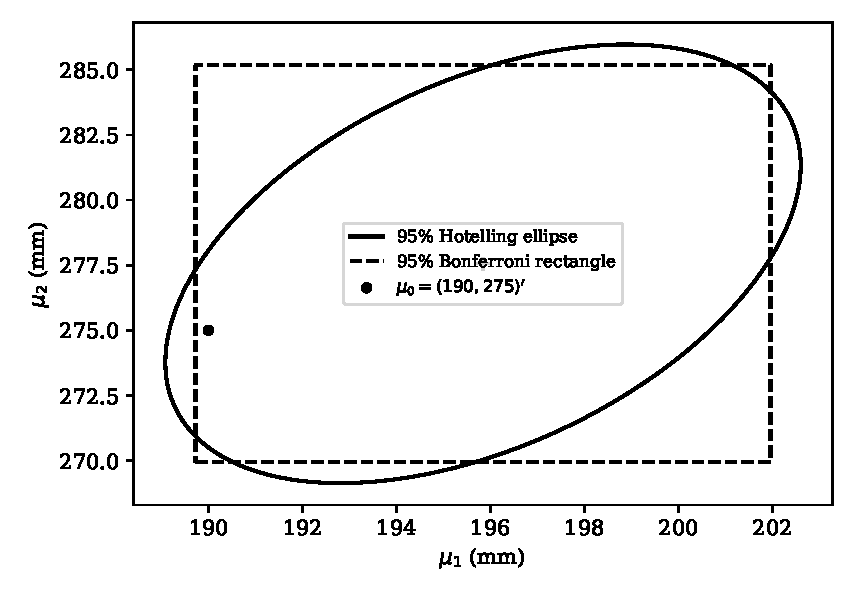
\includegraphics[width=0.74\linewidth]{figures/bai35_ellipse.pdf}
\end{center}
\item \textbf{Khoảng tin cậy đồng thời và so sánh.}\par\nopagebreak[4]
\step{1}{Xác định công thức và các hệ số.}
Với $j=1,2$, công thức hai loại khoảng là
\[
I_{T,j}=\bar{x}_j\pm\sqrt{c}\sqrt{s_{jj}/45},\qquad
I_{B,j}=\bar{x}_j\pm b\sqrt{s_{jj}/45}.
\]
Câu (a) cho $c\approx6.57847137$. Với Bonferroni, có $m=2$ đại lượng,
mỗi đuôi nhận $\alpha/(2m)=0.05/4=0.0125$. Vì vậy
\begin{align*}
n-1&=45-1=44,\\
1-\alpha/(2m)&=1-0.0125=0.9875,\\
b&=t_{44}(0.9875)\approx2.32071079.
\end{align*}
\step{2}{Tính từng khoảng $T^2$.}
\begin{samepage}
Với $j=1$, $\bar{x}_1\approx195.84444444$ và $s_{11}\approx312.81616162$:
\begin{align*}
\operatorname{SE}_{1}&=\sqrt{\frac{s_{11}}{n}}
=\sqrt{\frac{312.81616162}{45}}\approx2.63656410,\\
h_{1}&=\sqrt{6.57847137}\,2.6365641\approx6.76239958,\\
L_{1}&=\bar{x}_{1}-h_{1}
\approx 195.84444444-6.76239958=189.0820,\\
U_{1}&=\bar{x}_{1}+h_{1}
\approx 195.84444444+6.76239958=202.6068.
\end{align*}
\[
\answer{I_{T,1}=[189.0820,\;202.6068]}.
\]
\end{samepage}

\begin{samepage}
Với $j=2$, $\bar{x}_2\approx277.55555556$ và $s_{22}\approx484.2979798$:
\begin{align*}
\operatorname{SE}_{2}&=\sqrt{\frac{s_{22}}{n}}
=\sqrt{\frac{484.2979798}{45}}\approx3.28057576,\\
h_{2}&=\sqrt{6.57847137}\,3.28057576\approx8.41419488,\\
L_{2}&=\bar{x}_{2}-h_{2}
\approx 277.55555556-8.41419488=269.1414,\\
U_{2}&=\bar{x}_{2}+h_{2}
\approx 277.55555556+8.41419488=285.9698.
\end{align*}
\[
\answer{I_{T,2}=[269.1414,\;285.9698]}.
\]
\end{samepage}

\step{3}{Tính từng khoảng Bonferroni.}
\begin{samepage}
Với $j=1$, $\bar{x}_1\approx195.84444444$ và $s_{11}\approx312.81616162$:
\begin{align*}
\operatorname{SE}_{1}&=\sqrt{\frac{s_{11}}{n}}
=\sqrt{\frac{312.81616162}{45}}\approx2.63656410,\\
h_{1}&=2.32071079\cdot2.63656410\approx6.11870275,\\
L_{1}&=\bar{x}_{1}-h_{1}
\approx 195.84444444-6.11870275=189.7257,\\
U_{1}&=\bar{x}_{1}+h_{1}
\approx 195.84444444+6.11870275=201.9631.
\end{align*}
\[
\answer{I_{B,1}=[189.7257,\;201.9631]}.
\]
\end{samepage}

\begin{samepage}
Với $j=2$, $\bar{x}_2\approx277.55555556$ và $s_{22}\approx484.2979798$:
\begin{align*}
\operatorname{SE}_{2}&=\sqrt{\frac{s_{22}}{n}}
=\sqrt{\frac{484.2979798}{45}}\approx3.28057576,\\
h_{2}&=2.32071079\cdot3.28057576\approx7.61326756,\\
L_{2}&=\bar{x}_{2}-h_{2}
\approx 277.55555556-7.61326756=269.9423,\\
U_{2}&=\bar{x}_{2}+h_{2}
\approx 277.55555556+7.61326756=285.1688.
\end{align*}
\[
\answer{I_{B,2}=[269.9423,\;285.1688]}.
\]
\end{samepage}

Các khoảng đều có đơn vị mm.
\step{4}{So sánh độ dài hai loại khoảng.}
Độ dài bằng hai lần nửa độ rộng; cùng một biến có cùng sai số chuẩn nên
\begin{align*}
\frac{|I_{T,j}|}{|I_{B,j}|}
&=\frac{2\sqrt{c}\operatorname{SE}_j}{2b\operatorname{SE}_j}
=\frac{\sqrt{c}}b\\
&\approx\frac{2.56485309}{2.32071079}=1.105202,\\
\text{mức tăng tương đối}&=\left(\frac{\sqrt{c}}b-1\right)100\%
\approx10.52\%.
\end{align*}
Khoảng $T^2$ dài hơn cho cả hai trung bình.
\step{5}{Nêu ưu điểm của phương pháp $T^2$.}
Miền Hotelling bảo đảm đồng thời cho mọi tổ hợp tuyến tính
$\mathbf{a}'\boldsymbol{\mu}$ qua công thức
\[
\answer{\mathbf{a}'\boldsymbol{\mu}\in\mathbf{a}'\bar{\mathbf{x}}
\pm\sqrt{\frac{c\,\mathbf{a}'\mathbf{S}\mathbf{a}}{45}}},
\qquad\mathbf{a}\in\mathbb{R}^2.
\]
Do đó có thể chọn thêm hướng $\mathbf{a}$ sau khi xem dữ liệu.
Bonferroni với $m=2$ ở trên bảo đảm đồng thời cho hai trung bình đã định trước;
nếu chỉ cần hai trung bình này thì các khoảng Bonferroni ngắn hơn.
\end{enumerate}
\end{solution}

\begin{problem}[Bài 3.6.]
Mẫu gồm $n=61$ con gấu với sáu biến: cân nặng $X_1$ (kg), chiều dài cơ thể
$X_2$, chu vi vòng cổ $X_3$, chu vi vòng ngực $X_4$, chiều dài đầu $X_5$
và chiều rộng đầu $X_6$ (các chiều dài tính bằng cm). Cho
\[
\bar{\mathbf{x}}=(95.52,164.38,55.69,93.39,17.98,31.13)'
\]
và ma trận hiệp phương sai mẫu
\[
\mathbf{S}=\begin{pmatrix}
3266.46&1343.97&731.54&1175.50&162.68&238.37\\
1343.97&721.91&324.25&537.35&80.17&117.73\\
731.54&324.25&179.28&281.17&39.15&56.80\\
1175.50&537.35&281.17&474.98&63.73&94.85\\
162.68&80.17&39.15&63.73&9.95&13.88\\
238.37&117.73&56.80&94.85&13.88&21.16
\end{pmatrix}.
\]
\begin{enumerate}[label=(\alph*)]
\item Tìm khoảng tin cậy đồng thời $95\%$ cho sáu trung bình (mẫu lớn).
\item Xác định ellipse tin cậy $95\%$ cho trung bình cân nặng và chu vi vòng ngực
(mẫu lớn).
\item Tìm các khoảng Bonferroni $95\%$ cho sáu trung bình.
\item Xác định hình chữ nhật Bonferroni cho hai trung bình ở câu (b), dùng
$p=6$, và so sánh với ellipse.
\item Tìm khoảng Bonferroni $95\%$ cho hiệu trung bình chiều rộng đầu trừ
chiều dài đầu, với số đại lượng được xét là $6+1=7$.
\end{enumerate}
\end{problem}
\begin{solution}
Quy ước $m$ là số đại lượng cần bảo đảm đồng thời, còn $p$ là số chiều
của vectơ đang xét. Các phân vị được lấy theo xác suất tích lũy bên trái.
\begin{enumerate}[label=\textbf{\alph*)}]
\item \textbf{Khoảng tin cậy đồng thời mẫu lớn cho sáu trung bình.}\par\nopagebreak[4]
\step{1}{Xác định phân phối xấp xỉ và công thức khoảng.}
Với mẫu độc lập cùng phân phối, hiệp phương sai hữu hạn xác định dương
và $p=6$ cố định, định lý giới hạn trung tâm và Slutsky cho
\[
n(\bar{\mathbf{X}}-\boldsymbol{\mu})'\mathbf{S}^{-1}
(\bar{\mathbf{X}}-\boldsymbol{\mu})\xrightarrow{d}\chi_6^2.
\]
Chiếu miền này lên trục $j$ cho
\[
I_j=[\bar{x}_j-h_j,\bar{x}_j+h_j],\qquad
h_j=\sqrt{c_6}\operatorname{SE}_j,\quad
\operatorname{SE}_j=\sqrt{\frac{s_{jj}}n}.
\]
\step{2}{Tính phân vị tới hạn.}
Với $1-\alpha=1-0.05=0.95$, tra phân phối chi-bình phương có 6 bậc tự do:
\[
c_6=\chi_6^2(0.95)\approx12.59158724,\qquad
\sqrt{c_6}\approx3.54846266.
\]
\step{3}{Lấy phương sai từ đường chéo và tính sai số chuẩn.}
Dùng $n=61$; mỗi $s_{jj}$ lấy đúng vị trí hàng $j$, cột $j$ của ma trận đề:
\begin{center}
\small
\begin{tabular}{cccc}
\toprule
$j$ & $s_{jj}$ từ đề & Thế số $\operatorname{SE}_j$ & Kết quả\\
\midrule
$1$ & $3266.46$ & $\sqrt{3266.46/61}$ & $7.31768574$\\
$2$ & $721.91$ & $\sqrt{721.91/61}$ & $3.44014392$\\
$3$ & $179.28$ & $\sqrt{179.28/61}$ & $1.71435597$\\
$4$ & $474.98$ & $\sqrt{474.98/61}$ & $2.79044036$\\
$5$ & $9.95$ & $\sqrt{9.95/61}$ & $0.40387468$\\
$6$ & $21.16$ & $\sqrt{21.16/61}$ & $0.58896965$\\
\bottomrule
\end{tabular}
\end{center}

\step{4}{Tính nửa độ rộng, rồi hai cận cho cả sáu biến.}
Mỗi dòng áp dụng $h_j=\sqrt{c_6}\operatorname{SE}_j$ với cùng hệ số
$\sqrt{c_6}\approx3.54846266$:
\begin{center}
\small
\begin{tabular}{ccc}
\toprule
Biến & Thế số $h_j$ & Nửa độ rộng\\
\midrule
$1$ & $3.54846266\cdot7.31768574$ & $25.9665346$\\
$2$ & $3.54846266\cdot3.44014392$ & $12.20722223$\\
$3$ & $3.54846266\cdot1.71435597$ & $6.08332815$\\
$4$ & $3.54846266\cdot2.79044036$ & $9.9017734$\\
$5$ & $3.54846266\cdot0.40387468$ & $1.43313421$\\
$6$ & $3.54846266\cdot0.58896965$ & $2.0899368$\\
\bottomrule
\end{tabular}
\end{center}
Tiếp theo tính $L_j=\bar{x}_j-h_j$ và $U_j=\bar{x}_j+h_j$ cho từng biến:
\begin{center}
\small
\setlength{\tabcolsep}{4pt}
\begin{tabular}{ccc}
\toprule
Biến & Thế số cận dưới & Thế số cận trên\\
\midrule
$1$ & $95.52-25.9665346$ & $95.52+25.9665346$\\
$2$ & $164.38-12.20722223$ & $164.38+12.20722223$\\
$3$ & $55.69-6.08332815$ & $55.69+6.08332815$\\
$4$ & $93.39-9.9017734$ & $93.39+9.9017734$\\
$5$ & $17.98-1.43313421$ & $17.98+1.43313421$\\
$6$ & $31.13-2.0899368$ & $31.13+2.0899368$\\
\bottomrule
\end{tabular}
\end{center}
\begin{samepage}
Kết quả sau khi làm tròn bốn chữ số thập phân:
\begin{center}
\begin{tabular}{ccc}
\toprule
Tham số & Cận dưới $L_j$ & Cận trên $U_j$\\
\midrule
$\mu_1$ & $69.5535$ & $121.4865$\\
$\mu_2$ & $152.1728$ & $176.5872$\\
$\mu_3$ & $49.6067$ & $61.7733$\\
$\mu_4$ & $83.4882$ & $103.2918$\\
$\mu_5$ & $16.5469$ & $19.4131$\\
$\mu_6$ & $29.0401$ & $33.2199$\\
\bottomrule
\end{tabular}
\end{center}
\end{samepage}

\step{5}{Kết luận.}
Sáu khoảng $I_j=[L_j,U_j]$ ở bảng có độ bao phủ đồng thời xấp xỉ ít nhất
$95\%$ theo phương pháp mẫu lớn. Khoảng cho $\mu_1$ có đơn vị kg;
các khoảng còn lại có đơn vị cm.
\item \textbf{Ellipse cho trung bình cân nặng và vòng ngực.}\par\nopagebreak[4]
\step{1}{Chọn đúng hai thành phần của vectơ và ma trận.}
Cần xét $\boldsymbol{\theta}=(\mu_1,\mu_4)'$.
Lấy thành phần 1, 4 của trung bình và các hàng/cột 1, 4 của $\mathbf{S}$:
\[
\bar{\mathbf{x}}_{14}=\begin{pmatrix}95.52\\93.39\end{pmatrix},\qquad
\mathbf{S}_{14}=\begin{pmatrix}3266.46&1175.50\\1175.50&474.98\end{pmatrix}.
\]
Đặt $u=\mu_1-95.52$, $v=\mu_4-93.39$.
\step{2}{Xác định ngưỡng cho bài toán hai chiều.}
Xét riêng hai biến nên phân phối giới hạn có 2 bậc tự do.
Với mức $1-\alpha=0.95$:
\[
c_2=\chi_2^2(0.95)\approx5.99146455.
\]
Công thức miền là $61(u,v)\mathbf{S}_{14}^{-1}(u,v)'\le c_2$.
\step{3}{Tính nghịch đảo qua định thức.}

\begin{align*}
D_{14}&=3266.46\cdot474.98-(1175.50)^2\\
&=1551503.1708-1381800.2500=169702.9208.
\end{align*}
Do đó
\[
\mathbf{S}_{14}^{-1}=\frac1{169702.9208}
\begin{pmatrix}474.98&-1175.50\\-1175.50&3266.46\end{pmatrix}.
\]
Tính từng hệ số:
\begin{align*}
a&=474.98/169702.9208\approx0.002798891,\\
b&=-1175.50/169702.9208\approx-0.006926811,\\
c&=3266.46/169702.9208\approx0.019248107.
\end{align*}
\step{4}{Khai triển dạng toàn phương và kết luận.}
Tính trước $\mathbf{S}_{14}^{-1}(u,v)'=(au+bv,bu+cv)'$.
Nhân tiếp với $(u,v)$:
\begin{align*}
(u,v)\mathbf{S}_{14}^{-1}(u,v)'
&=u(au+bv)+v(bu+cv)\\
&=au^2+2buv+cv^2.
\end{align*}
Vì $2b\approx-0.013853621$, miền cần tìm có biểu thức số xấp xỉ
\[
\answer{61\left(0.002798891u^2-0.013853621uv
+0.019248107v^2\right)\le5.99146455}.
\]
Ellipse có tâm $(95.52,93.39)'$, nghiêng theo hướng tương quan dương
vì $s_{14}>0$.
Ở đây dùng 2 bậc tự do vì xét riêng cặp biến. Nếu chiếu miền sáu chiều
ở câu (a) xuống mặt phẳng này, cùng dạng toàn phương sẽ có ngưỡng
$c_6\approx12.59158724$; ellipse chiếu đó lớn hơn và giữ bảo đảm đồng thời
của bài toán sáu chiều.
\item \textbf{Khoảng Bonferroni cho sáu trung bình.}\par\nopagebreak[4]
\step{1}{Phân bổ mức sai lầm và chọn công thức.}
Có $m=6$ đại lượng cần xét. Mỗi khoảng hai phía nhận mức sai lầm
$\alpha/m=0.05/6$; mỗi đuôi nhận $\alpha/(2m)=0.05/12$.
Dùng công thức Student--Bonferroni
\[
I_{B,j}=\bar{x}_j\pm b_6\operatorname{SE}_j,\qquad
b_6=t_{n-1}\left(1-\frac{\alpha}{2m}\right).
\]
Công thức Student cho độ bao phủ chính xác của từng khoảng dưới giả thiết
chuẩn; nếu chỉ dùng giả thiết mẫu lớn thì các khoảng được hiểu là xấp xỉ.
\step{2}{Tính bậc tự do và phân vị.}
\begin{align*}
n-1&=61-1=60,\\
1-\frac{\alpha}{2m}&=1-\frac{0.05}{12}
=1-0.0041666667\approx0.9958333333,\\
b_6&=t_{60}(0.9958333333)\approx2.72855201.
\end{align*}
\step{3}{Tính nửa độ rộng và từng cận.}
Dùng lại sáu sai số chuẩn đã tính từ $\sqrt{s_{jj}/61}$ ở câu (a).
Mỗi nửa độ rộng là $h_{B,j}=b_6\operatorname{SE}_j$:
\begin{center}
\small
\begin{tabular}{ccc}
\toprule
Biến & Thế số $h_j$ & Nửa độ rộng\\
\midrule
$1$ & $2.72855201\cdot7.31768574$ & $19.9666861$\\
$2$ & $2.72855201\cdot3.44014392$ & $9.38661158$\\
$3$ & $2.72855201\cdot1.71435597$ & $4.67770942$\\
$4$ & $2.72855201\cdot2.79044036$ & $7.61386163$\\
$5$ & $2.72855201\cdot0.40387468$ & $1.10199306$\\
$6$ & $2.72855201\cdot0.58896965$ & $1.60703431$\\
\bottomrule
\end{tabular}
\end{center}
Tiếp theo tính $L_j=\bar{x}_j-h_j$ và $U_j=\bar{x}_j+h_j$ cho từng biến:
\begin{center}
\small
\setlength{\tabcolsep}{4pt}
\begin{tabular}{ccc}
\toprule
Biến & Thế số cận dưới & Thế số cận trên\\
\midrule
$1$ & $95.52-19.9666861$ & $95.52+19.9666861$\\
$2$ & $164.38-9.38661158$ & $164.38+9.38661158$\\
$3$ & $55.69-4.67770942$ & $55.69+4.67770942$\\
$4$ & $93.39-7.61386163$ & $93.39+7.61386163$\\
$5$ & $17.98-1.10199306$ & $17.98+1.10199306$\\
$6$ & $31.13-1.60703431$ & $31.13+1.60703431$\\
\bottomrule
\end{tabular}
\end{center}
\begin{samepage}
Kết quả sau khi làm tròn bốn chữ số thập phân:
\begin{center}
\begin{tabular}{ccc}
\toprule
Tham số & Cận dưới $L_j$ & Cận trên $U_j$\\
\midrule
$\mu_1$ & $75.5533$ & $115.4867$\\
$\mu_2$ & $154.9934$ & $173.7666$\\
$\mu_3$ & $51.0123$ & $60.3677$\\
$\mu_4$ & $85.7761$ & $101.0039$\\
$\mu_5$ & $16.8780$ & $19.0820$\\
$\mu_6$ & $29.5230$ & $32.7370$\\
\bottomrule
\end{tabular}
\end{center}
\end{samepage}

\step{4}{Kiểm tra độ bao phủ và so sánh độ dài.}
Gọi $A_j$ là biến cố khoảng thứ $j$ không chứa $\mu_j$.
Dưới giả thiết chuẩn, $P(A_j)=\alpha/m$, nên
\[
P(\text{cả sáu khoảng chứa đúng tham số})
\ge1-\sum_{j=1}^6P(A_j)
=1-6\frac{0.05}{6}=0.95.
\]
Tỷ lệ độ dài so với khoảng mẫu lớn ở câu (a) là
\[
\frac{2b_6\operatorname{SE}_j}{2\sqrt{c_6}\operatorname{SE}_j}
=\frac{b_6}{\sqrt{c_6}}
\approx\frac{2.72855201}{3.54846266}=0.768939<1.
\]
Vì vậy các khoảng Bonferroni ngắn hơn các khoảng ở câu (a).
\item \textbf{Hình chữ nhật Bonferroni và so sánh với ellipse.}\par\nopagebreak[4]
\step{1}{Lấy đúng hai khoảng, vẫn giữ hiệu chỉnh cho sáu đại lượng.}
Theo yêu cầu đề, giữ $m=6$ và hệ số $b_6$ ở câu (c), lấy $j=1,4$:
\begin{align*}
I_{B,1}&=[95.52-19.9666861,\;95.52+19.9666861],\\
I_{B,4}&=[93.39-7.61386163,\;93.39+7.61386163].
\end{align*}
Lấy tích Descartes để được miền chữ nhật:
\[
\answer{R_B=[75.5533,\;115.4867]
\times[85.7761,\;101.0039]}.
\]
\step{2}{Tính độ rộng chiếu của ellipse hai chiều.}
Với ellipse ở câu (b), nửa độ rộng chiếu lên trục $j$ là
$h_{E,j}=\sqrt{c_2}\operatorname{SE}_j$.
Thế $c_2\approx5.99146455$, $\sqrt{c_2}\approx2.44774683$:
\begin{align*}
h_{E,1}&\approx2.44774683\cdot7.31768574=17.91184208,\\
h_{E,4}&\approx2.44774683\cdot2.79044036=6.83029154.
\end{align*}
Do đó các khoảng chiếu của ellipse là
\begin{align*}
I_{E,1}&=[95.52-17.91184208,\;95.52+17.91184208]\\
&\approx[77.6082,\;113.4318],\\
I_{E,4}&=[93.39-6.83029154,\;93.39+6.83029154]\\
&\approx[86.5597,\;100.2203].
\end{align*}
\step{3}{Suy ra quan hệ bao hàm.}
Vì $2.44774683<2.72855201$, ta có
$h_{E,1}<h_{B,1}$ và $h_{E,4}<h_{B,4}$.
Các khoảng cùng tâm nên $I_{E,1}\subset I_{B,1}$ và
$I_{E,4}\subset I_{B,4}$. Mọi điểm trong ellipse thuộc cả hai khoảng chiếu,
vì vậy \textbf{ellipse hai chiều nằm hoàn toàn trong $R_B$}.
\begin{center}
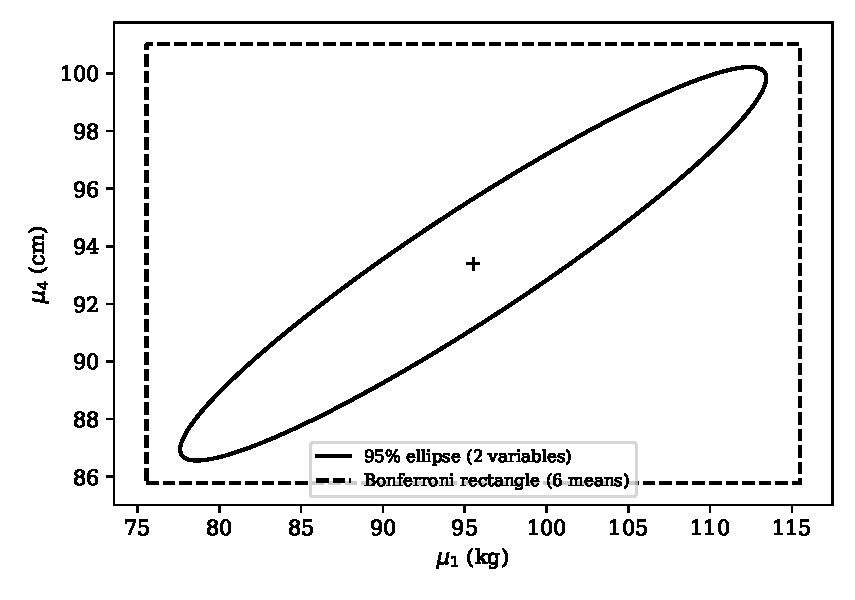
\includegraphics[width=0.74\linewidth]{figures/bai36_ellipse.pdf}
\end{center}
Ellipse tận dụng hiệp phương sai giữa hai biến. Hình chữ nhật cho phép đọc
cận từng trung bình trực tiếp, nhưng hiệu chỉnh cho sáu đại lượng nên bảo thủ hơn
khi chỉ xét cặp này. Quan hệ bao hàm ở đây dành cho ellipse hai chiều
ở câu (b), không phải ellipse chiếu từ miền sáu chiều.
\item \textbf{Khoảng Bonferroni cho hiệu $\mu_6-\mu_5$.}\par\nopagebreak[4]
\step{1}{Xác định đại lượng và trung bình mẫu.}
Đặt $D=X_6-X_5$; cần khoảng cho $\mathbb{E}[D]=\mu_6-\mu_5$.
Theo tính tuyến tính của trung bình mẫu:
\[
\bar{D}=\bar{x}_6-\bar{x}_5=31.13-17.98=13.15\text{ cm}.
\]
\step{2}{Khai triển phương sai của hiệu.}
Với hệ số $(1,-1)$, công thức là
\[
s_D^2=s_{66}+s_{55}-2s_{56}.
\]
Lấy từ ma trận đề $s_{66}=21.16$, $s_{55}=9.95$, $s_{56}=13.88$:
\begin{align*}
s_{66}+s_{55}&=21.16+9.95=31.11,\\
2s_{56}&=2\cdot13.88=27.76,\\
s_D^2&=31.11-27.76=3.35\text{ cm}^2.
\end{align*}
\step{3}{Tính sai số chuẩn của trung bình hiệu.}
\begin{align*}
\operatorname{SE}(\bar{D})&=\sqrt{\frac{s_D^2}n}\\
&=\sqrt{\frac{3.35}{61}}=\sqrt{0.0549180328}
\approx0.23434597\text{ cm}.
\end{align*}
\step{4}{Tính hệ số Bonferroni cho bảy đại lượng.}
Xét sáu trung bình và thêm một hiệu nên $m=6+1=7$;
cỡ mẫu vẫn là $n=61$, bậc tự do vẫn là $60$.
\begin{align*}
1-\frac{\alpha}{2m}&=1-\frac{0.05}{14}
=1-0.0035714286\approx0.9964285714,\\
b_7&=t_{60}(0.9964285714)\approx2.78546962.
\end{align*}
Để bảo đảm đồng thời cho cả bảy đại lượng, sáu khoảng trung bình đi kèm
cũng phải dùng $b_7$; hệ số $b_6$ ở câu (c) chỉ dành cho họ sáu đại lượng.
\step{5}{Tính nửa độ rộng và hai cận.}
Công thức là $\bar{D}\pm b_7\operatorname{SE}(\bar{D})$.
Thế số lần lượt:
\begin{align*}
h_D&=b_7\operatorname{SE}(\bar{D})
\approx2.78546962\cdot0.23434597=0.65276358,\\
L_D&=\bar{D}-h_D\approx13.15-0.65276358=12.4972,\\
U_D&=\bar{D}+h_D\approx13.15+0.65276358=13.8028.
\end{align*}
\step{6}{Kết luận.}
\[
\answer{\mu_6-\mu_5\in[12.4972,\;13.8028]\text{ cm}}.
\]
Đây là khoảng dùng hiệu chỉnh Bonferroni cho họ bảy đại lượng ở mức
đồng thời $95\%$; diễn giải hữu hạn mẫu chính xác cần giả thiết chuẩn,
còn theo bối cảnh mẫu lớn của bài thì độ bao phủ là xấp xỉ.
\end{enumerate}
\end{solution}

\end{document}
